\section{Conductividad a temperatura cero}
	
La conductividad a temperatura cero de este sistema se puede calcular mediante la formula de Kubo-Greenwood \autocite{Greenwood1958}
\begin{equation}\label{eq:KuboGreenwood}
	\sigma(E) = \frac{\pi \hbar e^2}{\Omega}\Trace[\delta(E - \widehat{H})\widehat{V}\delta(E - \widehat{H})\widehat{V}]
\end{equation}
donde $\Omega$ corresponde al volumen del sistema (en el caso de la cadena lineal $ \Omega = N $ el número de átomos en cadena), 
\begin{equation}\label{eq:trace}
	\Trace[\widehat{A}] = \frac{1}{N}\sum_n^N \bra{n}\widehat{A}\ket{n}
\end{equation}
corresponde a la traza (normalizada) sobre un conjunto base completo, $\delta(x)$ es la distribución de delta de Dirac y 
\begin{equation}\label{eq:VelocityOP}
	\widehat{V}_x = \frac{i}{\hbar} \comm{\widehat{H}}{\widehat{X}}
\end{equation}
es el operador velocidad en la dirección $x$; 
\begin{equation}\label{eq:comm}
	\comm{\widehat A}{\widehat B} = \widehat{A}\widehat{B} - \widehat{B}\widehat{A}
\end{equation}
es el conmutador de $\widehat{A}$ con $\widehat{B}$ y 
\begin{equation}\label{eq:positionOP}
	\widehat{X} = i \pdv{k_x}
\end{equation}
Es el operador velocidad en dirección $x$ escrito en la base del espacio recíproco.


Los elementos de matriz para el operador velocidad de la cadena lineal ($\widehat{V}_x = \widehat{V}$) quedan de la forma
\begin{align*}
	\matrixel{k}{\widehat{V}}{k'} &= \matrixel{k}{\frac{i}{\hbar} \comm{\widehat{H}}{\widehat{X}}}{k'}, \\
	\intertext{desarrollando el conmutador \eqref{eq:comm} y distribuyendo, se obtiene que}
	\matrixel{k}{\widehat{V}}{k'} &= \frac{i}{\hbar} \bqty{\matrixel{k}{\widehat{H}\widehat{X}}{k'} - \matrixel{k}{\widehat{X}\widehat{H}}{k'}}\\
	\intertext{cuya expasión dada por \eqref{eq:LC-TBHam} y \eqref{eq:positionOP} resulta en}
	\matrixel{k}{\widehat{V}}{k'} &= \frac{i}{\hbar} \bqty{\matrixel{k}{\sum_{q}\ketbra{q}\varepsilon(q)i\pdv{k}}{k'} - \matrixel{k}{i\pdv{k}\sum_{q}\ketbra{q}\varepsilon(q)}{k'}}\\
	\intertext{aplicando el ket $\bra{k}$ a la izquierda en el primer término y el ket $\ket{k'}$ en el segundo término, recordando que los vectores del número de ondas forman una base ortogonal, es decir $\braket{k}{q} = \delta^k_q$, entonces}
	\matrixel{k}{\widehat{V}}{k'} &= -\frac{1}{\hbar} \bqty{\matrixel{k}{\varepsilon(k)\pdv{k}}{k'} - \matrixel{k}{\pdv{k}\varepsilon(k')}{k'}},\\
	\intertext{el segundo término se desarrolla mediante la regla del producto,}
	\matrixel{k}{\widehat{V}}{k'} &= -\frac{1}{\hbar} \bqty{\matrixel{k}{\varepsilon(k)\pdv{k}}{k'} - \braket{k}{k'}\pdv{\varepsilon(k')}{k} - \matrixel{k}{\varepsilon(k)\pdv{k}}{k'}},\\
	\intertext{finalmente, eliminando términos iguales se obtiene}
	\matrixel{k}{\widehat{V}}{k'} &= \frac{1}{\hbar} \pdv{\varepsilon(k)}{k} \delta^{k'}_k = \frac{2t}{\hbar} a\sin(ka)\delta^{k'}_k . \numberthis\label{eq:velOPmatrixEl}
\end{align*}

Es posible aplicar distintos enfoques para calcular la traza de la conductividad de Kubo-Greenwood \eqref{eq:KuboGreenwood}, que se diferencian en la forma de abordar  los operadores de proyección cuánticos dentro de las mismas. Es de nuestro interés analizar la aproximación de estos operadores mediante el KPM y mediante funciones gausianas.

\subsection{Aproximación mediante el KPM}

Las deltas de Dirac se aproximan mediante el KPM \eqref{eq:kpm}
\begin{equation}\label{eq:diracDeltaKPM}
	\delta(E - \widehat{H}) \sim \frac{2}{\pi \Delta E \sqrt{1 - \widetilde{E}^2}} \sum_{m=0}^{M} T_m(\widetilde{E}) \frac{g^J_m T_m(\widetilde{H})}{1 + \delta^m_0},
\end{equation}
donde 
%\begin{equation*}\label{eq:bandWidth}
	$\Delta E = \frac{E_{\mathrm{máx}} - E_{\mathrm{mín}}}{2}$
%\end{equation*}
es el ancho de banda, 
%\begin{equation*}\label{eq:reducedEnergy}
	$\widetilde{E} = \frac{E - \bar{E}}{\Delta E}$ 
%\end{equation*}
es la energía reducida (y $\widetilde{H}$ es correspondientemente el hamiltoniano reducido), con $\bar{E} = \frac{E_{\mathrm{máx}} + E_{\mathrm{mín}}}{2}$ el centro de banda;
Se utiliza el kernel de Jackson, dado por los factores de amortiguamiento
\begin{equation}\label{eq:jacksonKernel}
	g_m^J = \frac{(M + 1 - m)\cos(\frac{\pi m}{M + 1}) + \sin(\frac{\pi m}{M + 1})\cot(\frac{\pi}{M + 1})}{M + 1},
\end{equation}
que ha demostrado ser óptimo para esta aplicación \autocite{Weise2006}.

Con todo lo anterior, la conductividad a temperatura cero se aproxima como
\begin{equation}\label{eq:KGapprox}
	\begin{aligned}
		\sigma(E) &\sim \frac{4\hbar e^2}{\pi\Omega{\Delta E}^2(1 - \widetilde{E}^2)} \sum_{m=0}^{M} \sum_{n=0}^{M} T_m(\widetilde{E})T_n(\widetilde{E}) g^J_m g^J_n \frac{\Trace[T_m(\widetilde{H})\widehat{V}T_n(\widetilde{H})\widehat{V}]}{(1 + \delta^m_0) (1 + \delta^n_0)}, \\ 
		\sigma(E) &\sim \frac{4\hbar e^2}{\pi\Omega{\Delta E}^2(1 - \widetilde{E}^2)} \sum_{m=0}^{M} \sum_{n=0}^{M} T_m(\widetilde{E})T_n(\widetilde{E}) g^J_m g^J_n \mu^m_n,
	\end{aligned}
\end{equation}
de modo que es de interés analizar la traza en la expresión anterior para el caso específico de la cadena lineal.

Para los próximos análisis se asume una amplitud de salto entre vecinos cercanos $t = -½$, dado esto, las auto-energías, dadas por la función $ E(k) = \varepsilon(E) \stackrel{t = -½}{=} \cos(ka) $, están acotadas por los valores $ E_{\mathrm{máx}} = 1 $ y $ E_{\mathrm{mín}} = -1 $, por lo tanto se tiene que $ \Delta E = 1 $, $ \bar{E} = 0 $, lo cuál implica que $ \widetilde{E} = E $ y $ \widetilde{H} = \widehat{H} $. De modo que la traza, desarrollada según \eqref{eq:trace}, queda de la forma
\begin{align*}
	\Trace[T_m(\widetilde{H})\widehat{V}T_n(\widetilde{H})\widehat{V}] &= \frac{1}{N}\sum_{k} \expval{T_m(\widehat{H})\widehat{V}T_n(\widehat{H})\widehat{V}}{k}; \\
	\intertext{para cualquier función $ f $ expandible en serie de potencias, se tiene que $f(\widehat{H}) = \sum_{k} \ketbra{k} f(\varepsilon)$. Para los polinomios de Chebyshev $ T_m(\widehat{H}) = \sum_{k} \ketbra{k} T_m(\varepsilon) = \sum_{k} \ketbra{k} \cos(mka) $, dada la expresión de los polinomios de Chebyshev \eqref{eq:ChebyshevPol}, así que}
	\Trace[T_m(\widetilde{H})\widehat{V}T_n(\widetilde{H})\widehat{V}] &= \frac{1}{N}\sum_{k} \expval{\sum_{k'}\ketbra{k'} \cos(mk'a)\widehat{V}T_n(\widehat{H})\widehat{V}}{k}, \\
	\intertext{aprovechando la relación de completitud \eqref{eq:k-completness}, entonces}
	\Trace[T_m(\widetilde{H})\widehat{V}T_n(\widetilde{H})\widehat{V}] &= \frac{1}{N}\smashoperator{\sum_{k,q,q'}} \bra{k}{\sum_{k'}\ketbra{k'} \cos(mk'a)\ket{q}\bra{q}\widehat{V}\ket{q'}\bra{q'}T_n(\widehat{H})\widehat{V}}{k}\ket{k}, \\
	\intertext{aplicando el $\bra{k}$ por la derecha y expandiendo los elementos de matriz para el operador velocidad \eqref{eq:velOPmatrixEl} se obtiene}
	\Trace[T_m(\widetilde{H})\widehat{V}T_n(\widetilde{H})\widehat{V}] &= -\frac{a}{\hbar N} \sum_{k,q} \bra{k} \ket{q}\cos(mka)\sin(qa)\bra{q}T_n(\widehat{H})\widehat{V}\ket{k}, \\
	\Trace[T_m(\widetilde{H})\widehat{V}T_n(\widetilde{H})\widehat{V}] &= -\frac{a}{\hbar N} \sum_{k} \cos(mka)\sin(ka)\bra{k}T_n(\widehat{H})\widehat{V}\ket{k}, \\
	\intertext{aplicando el mismo procedimiento para el elemento de matriz faltante, da}
	\Trace[T_m(\widetilde{H})\widehat{V}T_n(\widetilde{H})\widehat{V}] &= \pqty{\frac{a}{\hbar}}^2 \frac{1}{N} \sum_{k} \sin[2](ka)\cos(mka)\cos(nka). \\
	\intertext{Adicionalmente se le establecen condiciones de frontera períodica a la cadena lineal, de modo que las auto-energías se cuantizan a aquellas correspodientes a los valores del vector de onda $ak_n = \frac{2\pi n}{N}$, con $ N $ el número de átomos en la cadena y el índice entero $ n $ va de 0 a $N$. Con esto se puede transformar la sumatoria en una integral sobre el espacio-k mediante la definición de la suma de Riemman}
	\Trace[T_m(\widetilde{H})\widehat{V}T_n(\widetilde{H})\widehat{V}] &= \pqty{\frac{a}{\hbar}}^2 \frac{N}{2\pi N} \smashoperator{\int_{0}^{2\pi}} \sin[2](ka)\cos(mka)\cos(nka)d(ka).\label{eq:chebMomTraceInt}\numberthis \\ 
	\intertext{Resolviendo la integral \apdref{ap:chebMomTraceInt},}
	\Trace[T_m(\widehat{H})\widehat{V}T_n(\widehat{H})\widehat{V}] &= \pqty{\frac{a}{\hbar}}^2 \frac{1}{2\pi} \frac{\pi}{2} \bqty{\delta^m_n(1 + \delta^m_0)(1-\tfrac{1}{2}\delta^m_1) - \tfrac{1}{2}(1 - \delta^m_n)(\delta^{m+n}_2 + \delta^{\abs{m-n}}_2)},
\end{align*}
con esto se puede obtener la cantidad $ \mu^m_n $, presentada en la expresión \eqref{eq:KGapprox},
\begin{align*}
	\mu^m_n &= \pqty{\frac{a}{2\hbar}}^2 \bqty{\delta^m_n\frac{(1 + \delta^m_0)(1-\tfrac{1}{2}\delta^m_1)}{(1 + \delta^m_0)^2} - \tfrac{1}{2}(1 - \delta^m_n)\frac{\delta^{m+n}_2 + \delta^{\abs{m-n}}_2}{(1 + \delta^m_0) (1 + \delta^n_0)}},\\
	\mu^m_n &= \pqty{\frac{a}{2\hbar}}^2 \bqty{\delta^m_n\frac{(1-\tfrac{1}{2}\delta^m_1)}{(1 + \delta^m_0)}\frac{1 + \delta^m_1}{1 + \delta^m_1} - \tfrac{1}{2}(1 - \delta^m_n)\frac{\delta^{m+n}_2 + \delta^{\abs{m-n}}_2}{(1 + \delta^m_0) (1 + \delta^n_0)} \frac{1 - \tfrac{1}{2}\delta^m_0 - \tfrac{1}{2}\delta^n_0}{1 - \tfrac{1}{2}\delta^m_0 - \tfrac{1}{2}\delta^n_0}},\\
	\intertext{Para $ m \neq n $ la ecuación $ m + n = 2 $ solo tiene como resultados posibles los valores $ (m, n) = \{(0, 2), (2, 0)\} $ por lo cual $ \delta^{m+n}_2 = \delta^m_0\delta^n_2 + \delta^m_2\delta^n_0 $,}
	\mu^m_n &= \pqty{\frac{a}{2\hbar}}^2 \bqty{\frac{\delta^m_n}{(1 + \delta^m_0 + \delta^m_1)} - \tfrac{1}{2}(1 - \delta^m_n)(\delta^m_0\delta^n_2 + \delta^m_2\delta^n_0 + \delta^{\abs{m-n}}_2)(1 - \tfrac{1}{2}\delta^m_0 - \tfrac{1}{2}\delta^n_0)},\\
	\mu^m_n &= \pqty{\frac{a}{2\hbar}}^2 \bqty{\frac{\delta^m_n}{(1 + \delta^m_0 + \delta^m_1)} - \tfrac{1}{2}(1 - \delta^m_n)\delta^{\abs{m-n}}_2}.\numberthis\label{eq:LC_KPM_moments}
\end{align*}

Sustituyendo esta expresión en la aproximación para la conductividad \eqref{eq:KGapprox}
\begin{align*}
	\sigma(E) &\sim \frac{4\hbar e^2}{N\pi(1 - E^2)} \pqty{\frac{a}{2\hbar}}^2 \sum_{m=0}^{M} \sum_{n=0}^{M} T_m(E)T_n(E)g_m g_n \bqty{\frac{\delta^m_n}{(1 + \delta^m_0 + \delta^m_1)} - \tfrac{1}{2}(1 - \delta^m_n)\delta^{\abs{m-n}}_2},\\
	\sigma(E) &\sim \frac{a^2e^2}{Nh(1 - E^2)} \sum_{m=0}^{M} \sum_{n=0}^{M} T_m(E)T_n(E)g_m g_n \bqty{\frac{\delta^m_n}{(1 + \delta^m_0 + \delta^m_1)} - \tfrac{1}{2}(1 - \delta^m_n)\delta^{\abs{m-n}}_2}.\numberthis
\end{align*}

\subsection{Aproximación mediante función Gaussiana}\label{ssec:aproxGauss}

Para empezar, nos aprovechamos de que tanto el operador velocidad y el operador de proyección cuántico son diagonales en el espacio de momentos, tal que la traza de \eqref{eq:KuboGreenwood} se puede expresar como
\begin{align*}
	\Tr[\delta(E - \widehat{H}) \widehat{V} \delta(E - \widehat{H}) \widehat{V}] &= \frac{1}{N} \sum_{k} \bra{k} \delta(E - \widehat{H}) \widehat{V} \delta(E - \widehat{H}) \widehat{V} \ket{k}, \\ 
	\intertext{Aplicando relaciones de completitud, nos quedamos con los autovalores de $ \widehat{H} $ \eqref{eq:LC-kHAM} y $ \widehat{V} $ \eqref{eq:velOPmatrixEl}}
	\Tr[\delta(E - \widehat{H}) \widehat{V} \delta(E - \widehat{H}) \widehat{V}] &= \frac{4t^2a^2}{N \hbar^2}\sum_{k} \delta^2(E + 2t\cos(ka)) \sin[2](ka).
\end{align*}

La aproximación pertinente resulta entonces en aproximar uno de los operadores de proyección mediante una función Gaussiana
\begin{equation*}
	\delta(E + 2t\cos(ka)) = \lim_{\sigma \to 0} \frac{1}{\sqrt{2\pi\sigma^2}}\exp(-\frac{[E + 2t\cos(ka)]^2}{2\sigma^2}),
\end{equation*}
donde sigma se interpreta como un ensanchamiento de las energías permitidas por el operador de proyección, de modo que, cambiando la sumatoria de la traza por una integral sobre el espacio de momentos, obtenemos la expresión
\begin{align*}
	\Tr[\cdots] &= \frac{4t^2a^2}{2 \pi\hbar^2\sqrt{2\pi\sigma^2}} \int_{0}^{2\pi} \exp(-\frac{[E + 2t\cos(ka)]^2}{2\sigma^2}) \sin[2](ka) \delta(E + 2t\cos(ka)) d(ka), \\ 
	\Tr[\cdots] &= \frac{2t^2a^2}{\pi\hbar^2\sqrt{2\pi\sigma^2}} \sum_{i} \exp(-\frac{[E + 2t\cos(k_ia)]^2}{2\sigma^2}) \frac{\sin[2](k_ia)}{\abs{2ta\sin(k_ia)}}, \\ 
	\Tr[\cdots] &= \frac{|t|a}{\pi\hbar^2\sqrt{2\pi\sigma^2}} \sum_{i} \exp(-\frac{[E + 2t\cos(k_ia)]^2}{2\sigma^2}) \abs{\sin(k_ia)}, \\
	\Tr[\cdots] &= \frac{2|t|a}{\pi\hbar^2\sqrt{2\pi\sigma^2}} \exp(-\frac{[E - E]^2}{2\sigma^2}) \abs{\sin(\acos(-\frac{E}{2t}))}, \\ 
	\Tr[\cdots] &= \frac{2|t|a}{\pi\hbar^2\sqrt{2\pi\sigma^2}} \sqrt{1 - \frac{E^2}{4t^2}} = \frac{a}{\pi\hbar^2\sqrt{2\pi\sigma^2}} \sqrt{4t^2 - E^2}\numberthis.
\end{align*}

Finalmente, sustituyendo esta expresión en la conductividad a temperatura cero resulta en

\begin{equation}\label{eq:kuboBastinGauss}
	\sigma(E, \mu) = \frac{a e^2}{N} \frac{a}{\hbar\sqrt{2\pi\mu^2}} \sqrt{4t^2 - E^2}
\end{equation}

\begin{figure}[bt]
	\centering
	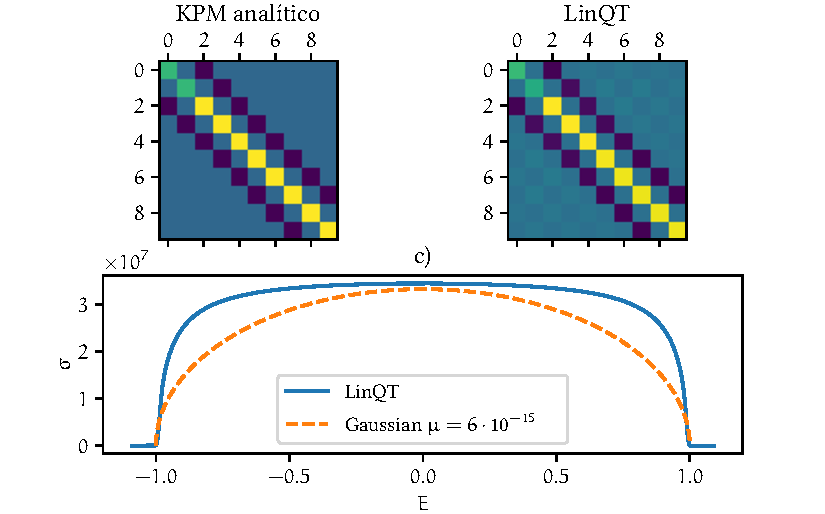
\includegraphics{./img/LC_cond.pdf}
	\caption{Resultados obtenidos para la conductividad a temperatura cero de la cadena lineal mono-atómica ($ N = 2\cdot\megad $) según la ecuación de Kubo-Greenwood \eqref{eq:KuboGreenwood}. Se muestran los primeros $ 10 \times 10 $ elementos de la matriz de momentos $ \mu $ de la aproximación mediante KPM \eqref{eq:KGapprox} calculados de forma analítica bajo la expresión \eqref{eq:LC_KPM_moments} y mediante el programa \textsc{LinQT}, a su vez que se observa la conductividad $ \sigma $ obtenida tanto por \textsc{LinQT} como la aproximación del operador de proyección usando una función Gaussiana \eqref{eq:kuboBastinGauss}. \label{fig:LC_cond}}
\end{figure}